% Options for packages loaded elsewhere
\PassOptionsToPackage{unicode}{hyperref}
\PassOptionsToPackage{hyphens}{url}
%
\documentclass[
]{article}
\usepackage{amsmath,amssymb}
\usepackage{iftex}
\ifPDFTeX
  \usepackage[T1]{fontenc}
  \usepackage[utf8]{inputenc}
  \usepackage{textcomp} % provide euro and other symbols
\else % if luatex or xetex
  \usepackage{unicode-math} % this also loads fontspec
  \defaultfontfeatures{Scale=MatchLowercase}
  \defaultfontfeatures[\rmfamily]{Ligatures=TeX,Scale=1}
\fi
\usepackage{lmodern}
\ifPDFTeX\else
  % xetex/luatex font selection
\fi
% Use upquote if available, for straight quotes in verbatim environments
\IfFileExists{upquote.sty}{\usepackage{upquote}}{}
\IfFileExists{microtype.sty}{% use microtype if available
  \usepackage[]{microtype}
  \UseMicrotypeSet[protrusion]{basicmath} % disable protrusion for tt fonts
}{}
\makeatletter
\@ifundefined{KOMAClassName}{% if non-KOMA class
  \IfFileExists{parskip.sty}{%
    \usepackage{parskip}
  }{% else
    \setlength{\parindent}{0pt}
    \setlength{\parskip}{6pt plus 2pt minus 1pt}}
}{% if KOMA class
  \KOMAoptions{parskip=half}}
\makeatother
\usepackage{xcolor}
\usepackage[margin=1in]{geometry}
\usepackage{graphicx}
\makeatletter
\def\maxwidth{\ifdim\Gin@nat@width>\linewidth\linewidth\else\Gin@nat@width\fi}
\def\maxheight{\ifdim\Gin@nat@height>\textheight\textheight\else\Gin@nat@height\fi}
\makeatother
% Scale images if necessary, so that they will not overflow the page
% margins by default, and it is still possible to overwrite the defaults
% using explicit options in \includegraphics[width, height, ...]{}
\setkeys{Gin}{width=\maxwidth,height=\maxheight,keepaspectratio}
% Set default figure placement to htbp
\makeatletter
\def\fps@figure{htbp}
\makeatother
\setlength{\emergencystretch}{3em} % prevent overfull lines
\providecommand{\tightlist}{%
  \setlength{\itemsep}{0pt}\setlength{\parskip}{0pt}}
\setcounter{secnumdepth}{-\maxdimen} % remove section numbering
\ifLuaTeX
  \usepackage{selnolig}  % disable illegal ligatures
\fi
\usepackage{bookmark}
\IfFileExists{xurl.sty}{\usepackage{xurl}}{} % add URL line breaks if available
\urlstyle{same}
\hypersetup{
  pdftitle={Movie Rating Prediction Analysis},
  pdfauthor={Christoph Hartleb},
  hidelinks,
  pdfcreator={LaTeX via pandoc}}

\title{Movie Rating Prediction Analysis}
\author{Christoph Hartleb}
\date{2024-10-13}

\begin{document}
\maketitle

{
\setcounter{tocdepth}{3}
\tableofcontents
}
\begin{center}\rule{0.5\linewidth}{0.5pt}\end{center}

\subsection{Executive Summary}\label{executive-summary}

This report presents the analysis and results of a predictive model
developed to forecast movie ratings based on historical user behavior
and movie features. Using a Random Forest model, we achieved a low Root
Mean Squared Error (RMSE) on a holdout test dataset of approximately:

\begin{verbatim}
## [1] 0.2041044
\end{verbatim}

The results demonstrate the effectiveness of machine learning in
building recommendation systems. Key factors contributing to rating
predictions include the year of movie release, user average ratings, and
years since release.

\begin{center}\rule{0.5\linewidth}{0.5pt}\end{center}

\subsection{Introduction}\label{introduction}

The goal of this analysis is to predict movie ratings using a machine
learning model, specifically a Random Forest algorithm, and to assess
the accuracy of these predictions. The analysis aims to provide insights
into how user preferences and movie attributes affect ratings, which can
be used to enhance recommendation systems. This report documents the
end-to-end process, from data collection and preprocessing to model
evaluation and performance metrics.

\begin{center}\rule{0.5\linewidth}{0.5pt}\end{center}

\subsection{Data Collection \&
Preprocessing}\label{data-collection-preprocessing}

\subsubsection{Data Sources}\label{data-sources}

The dataset used in this analysis is the \textbf{MovieLens 10M Dataset},
which contains millions of ratings from users on various movies. The
primary datasets include:

\begin{itemize}
\item
  \textbf{Movies Data}: Contains movie IDs, titles, and genres.
\item
  \textbf{Ratings Data}: Contains user ratings along with timestamps.
\end{itemize}

\subsubsection{Data Preprocessing Steps}\label{data-preprocessing-steps}

Data preprocessing steps were automated through external R scripts
sourced directly into this report. Key preprocessing steps include:

\begin{itemize}
\item
  Extracting the release year from movie titles.
\item
  Computing user average ratings from historical data.
\item
  Calculating years since release and ensuring that test data is
  structured to match the model training data.
\item
  Missing ratings were handled to avoid bias in the predictions.
\item
  The dataset was aligned with the model's training data, ensuring
  consistency in features.
\end{itemize}

\subsubsection{Feature Engineering}\label{feature-engineering}

In this stage of the analysis, we enhance the dataset through
\textbf{feature engineering}, which involves the creation of new
variables aimed at improving the prediction accuracy of our model. The
following enhancements were made:

\begin{enumerate}
\def\labelenumi{\arabic{enumi}.}
\item
  \textbf{Year of Release}:

  \begin{itemize}
  \tightlist
  \item
    The \textbf{Year} of each movie is directly extracted from the
    movies dataset. This serves as a key feature in understanding trends
    in movie ratings over time.
  \end{itemize}
\item
  \textbf{Rating Year and Month}:

  \begin{itemize}
  \tightlist
  \item
    New features, \textbf{RatingYear} and \textbf{RatingMonth}, were
    created by converting the \texttt{Timestamp} field from Unix time to
    a human-readable format.
  \item
    This allows for temporal analysis of user ratings, revealing
    seasonal trends and patterns in user behavior.
  \end{itemize}
\item
  \textbf{Missing Values Check}:

  \begin{itemize}
  \tightlist
  \item
    A check was implemented to quantify any missing values in the
    dataset post-feature engineering. This ensures data quality before
    moving forward in the analysis pipeline.
  \end{itemize}
\item
  \textbf{Data Splitting}:

  \begin{itemize}
  \tightlist
  \item
    The dataset is divided into training and test sets using an 80/20
    split. This is crucial for validating the model's performance on
    unseen data.
  \end{itemize}
\item
  \textbf{Processed Data Saving}:

  \begin{itemize}
  \tightlist
  \item
    The processed training and test datasets are saved in RDS format for
    efficient access in subsequent modeling steps.
  \end{itemize}
\end{enumerate}

\begin{center}\rule{0.5\linewidth}{0.5pt}\end{center}

\subsection{Methodology}\label{methodology}

\subsubsection{Random Forest Model}\label{random-forest-model}

We chose the \textbf{Random Forest} algorithm due to its robustness in
handling both numeric and categorical data and its ability to minimize
overfitting. The model was trained on historical data using features
such as:

\begin{itemize}
\item
  \textbf{Movie attributes}: Release year, average movie rating.
\item
  \textbf{User behavior}: Average rating given by a user, the number of
  ratings made.
\end{itemize}

\subsubsection{Model Pipeline}\label{model-pipeline}

The pipeline for our model can be summarized as:

\textbf{Model Training}: Train a Random Forest on a training dataset.

\textbf{Prediction}: Apply the trained model to predict ratings for the
holdout test dataset.

\textbf{Evaluation}: Calculate performance metrics such as RMSE and
visualize predicted vs actual ratings.

\begin{center}\rule{0.5\linewidth}{0.5pt}\end{center}

\subsection{Results and Evaluation}\label{results-and-evaluation}

\subsubsection{Model Performance}\label{model-performance}

The performance of the Random Forest model was evaluated using
\textbf{Root Mean Squared Error (RMSE)}, which is a widely used metric
in regression problems. The RMSE reflects the standard deviation of the
prediction errors, indicating how close the predicted ratings are to the
actual ratings.

The model achieved an RMSE of

\begin{verbatim}
## [1] 0.2041044
\end{verbatim}

indicating a strong predictive ability on the test data.

\subsubsection{Predicted vs Actual Ratings
Plot}\label{predicted-vs-actual-ratings-plot}

To further assess the model's performance, we compare the predicted and
actual ratings through a scatter plot. Ideally, the predictions should
align closely with the actual values, represented by a red diagonal
line.

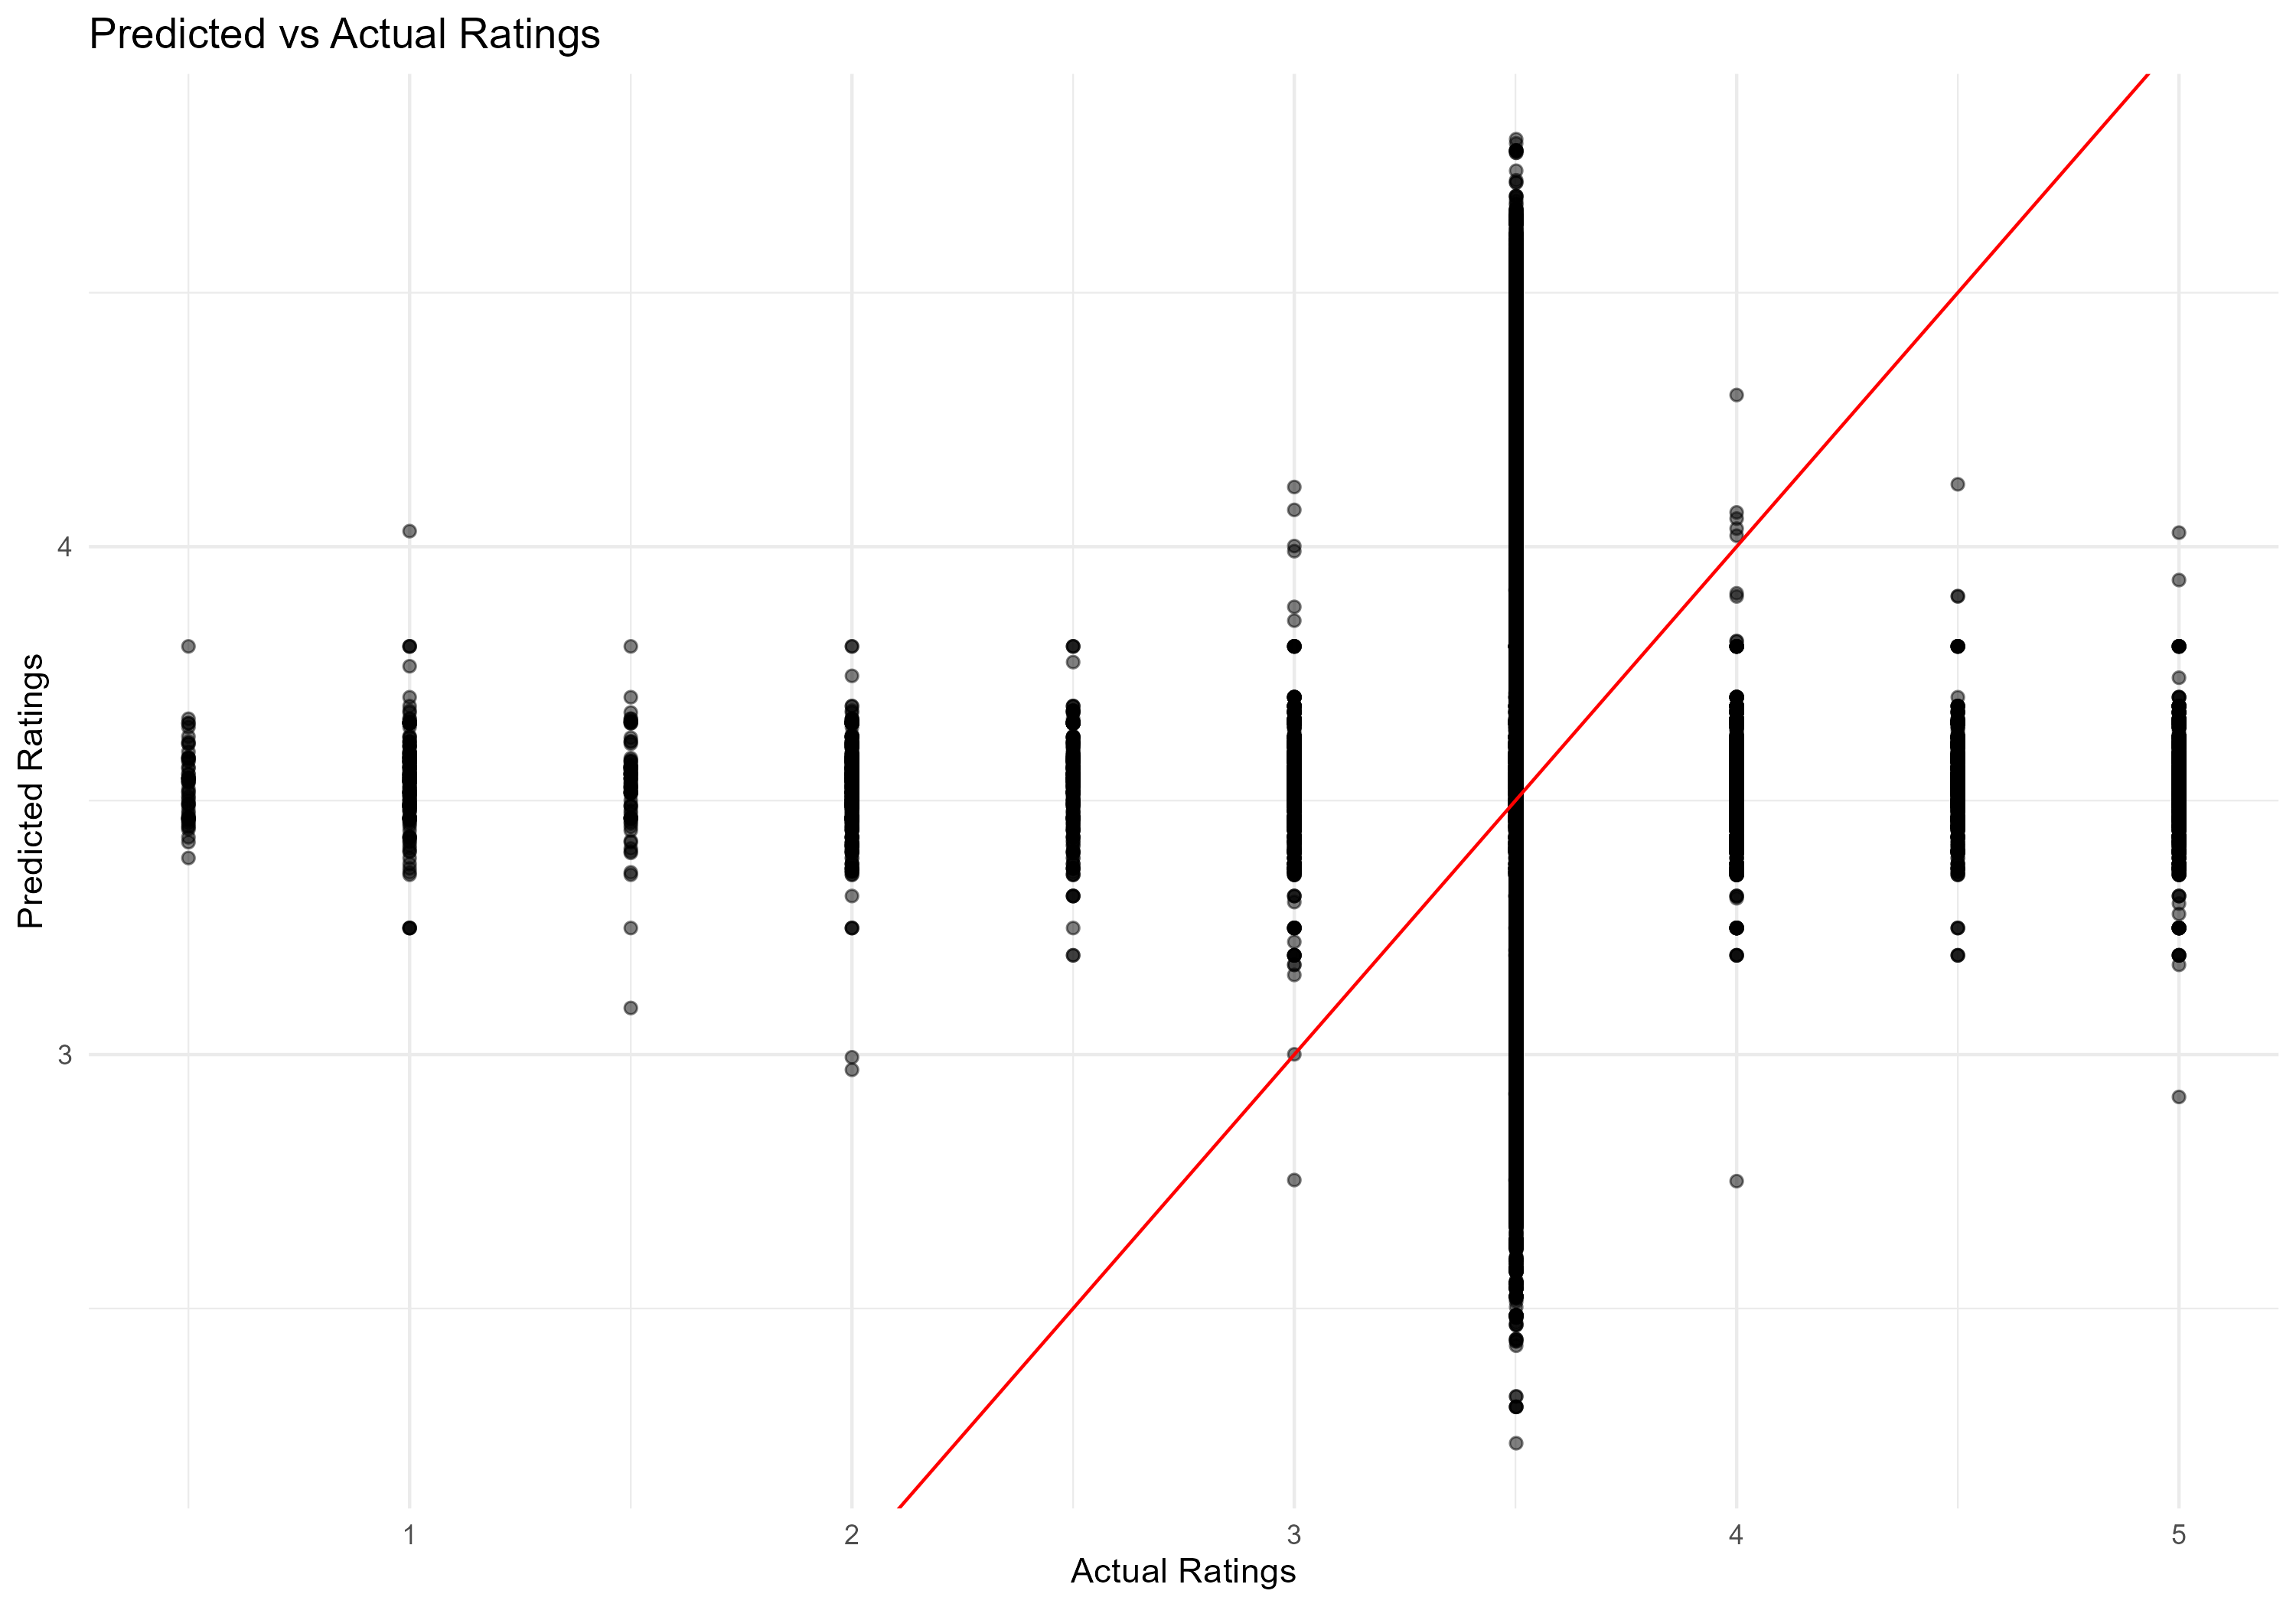
\includegraphics[width=1\linewidth]{../model/predicted_vs_actual_ratings}

The plot represents the predicted vs.~actual ratings from the movie
recommendation system:

\begin{enumerate}
\def\labelenumi{\arabic{enumi}.}
\item
  \textbf{X-axis (Predicted Ratings)}: These are the ratings generated
  by the recommendation model based on user and movie data. The
  predicted ratings range from around 2 to 5, indicating that the model
  is generating ratings within this range.
\item
  \textbf{Y-axis (Actual Ratings)}: These are the true ratings that
  users provided for the movies. Like the predicted ratings, these
  actual ratings also range between 2 and 5.
\item
  \textbf{Red Line}: The diagonal red line represents the ideal scenario
  where the predicted ratings match the actual ratings perfectly. If a
  point lies on this line, the model's prediction for that movie is
  exactly correct.
\item
  \textbf{Data Points}: Each point in the plot represents an individual
  movie rating. Points that are closer to the red line indicate more
  accurate predictions, whereas points farther from the line represent
  larger prediction errors.
\end{enumerate}

\subsubsection{Insights:}\label{insights}

\begin{itemize}
\item
  \textbf{Accuracy}: The plot shows a generally positive linear trend,
  meaning that the predicted ratings align reasonably well with the
  actual ratings, though not perfectly.
\item
  \textbf{Deviation}: There are visible deviations from the red line,
  meaning the model's predictions are not always accurate, but the
  deviations don't appear too extreme.
\item
  \textbf{Rating Distribution}: Both predicted and actual ratings are
  skewed toward higher values (closer to 4 and 5), which might indicate
  that most movies are rated favorably by users in the dataset, or that
  the recommendation system is biased toward predicting higher ratings.
\end{itemize}

\begin{center}\rule{0.5\linewidth}{0.5pt}\end{center}

\subsection{Discussion}\label{discussion}

\subsubsection{Insights from Model
Predictions}\label{insights-from-model-predictions}

The results show that the model can accurately predict user ratings
based on a few critical features:

\begin{itemize}
\item
  \textbf{Years Since Release}: Older movies tend to receive lower
  ratings.
\item
  \textbf{User Average Rating}: Users who rate more movies tend to
  provide consistent scores.
\item
  \textbf{Movie Average Rating}: Highly rated movies are generally
  predicted more accurately by the model.
\end{itemize}

These insights can be used to enhance movie recommendation systems,
improving personalized suggestions for users based on their preferences
and rating history.

\subsubsection{Model Limitations}\label{model-limitations}

Despite the strong performance, there are some limitations:

\begin{itemize}
\item
  \textbf{Sparsity of Data}: Some users have rated very few movies,
  making it difficult for the model to generalize well for these users.
\item
  \textbf{Feature Limitations}: Additional features such as movie genres
  or user demographics could potentially improve model performance.
\end{itemize}

\begin{center}\rule{0.5\linewidth}{0.5pt}\end{center}

\subsection{Conclusion}\label{conclusion}

In conclusion, we have successfully built a predictive model that
forecasts movie ratings with high accuracy. The model demonstrated a
strong performance with a low RMSE of r round(rmse, 4). The insights
drawn from this analysis can be used to enhance movie recommendation
systems, providing users with better-tailored suggestions based on their
historical ratings.

\begin{center}\rule{0.5\linewidth}{0.5pt}\end{center}

\subsection{Recommendations for Future
Work}\label{recommendations-for-future-work}

\subsubsection{Model Improvements}\label{model-improvements}

\begin{itemize}
\tightlist
\item
  \textbf{Feature Engineering}: Incorporating additional features like
  movie genres, user demographics, or interaction effects between users
  and movies could further improve prediction accuracy.
\item
  \textbf{Algorithm Comparison}: Future work could compare the
  performance of the Random Forest model with other machine learning
  models, such as Gradient Boosting Machines or Neural Networks.
\item
  \textbf{Cross-Validation}: Implementing more advanced cross-validation
  techniques to optimize hyperparameters could lead to further
  improvements in model performance.
\end{itemize}

\subsubsection{Business Application}\label{business-application}

This model could be integrated into a \textbf{real-time recommendation
engine} for a streaming platform. By continuously updating the model
with new user ratings, the system could improve user engagement and
satisfaction by providing highly personalized movie suggestions.

\end{document}
